\documentclass[border=2pt]{standalone}
\usepackage{pgfplots}\pgfplotsset{compat=1.18}\usepackage{amsmath}
\begin{document}
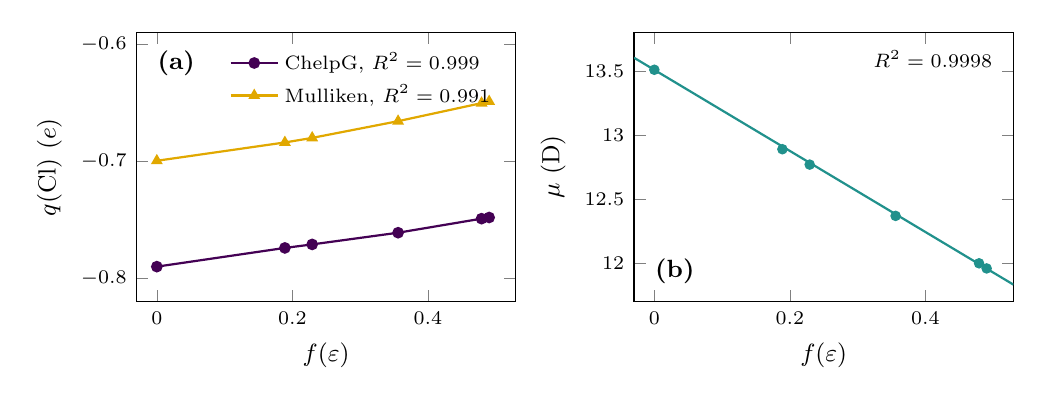
\begin{tikzpicture}
  \definecolor{c1}{HTML}{440154}\definecolor{c2}{HTML}{21918C}\definecolor{c3}{HTML}{E1A800}
  \pgfplotsset{every axis/.append style={width=6.4cm,height=5cm,
    tick label style={font=\scriptsize},label style={font=\small},
    tick align=inside,mark size=1.7pt,
    legend style={font=\scriptsize,draw=none,fill=none},legend cell align=left}}

  \begin{axis}[name=a, xlabel={$f(\varepsilon)$}, ylabel={$q$(Cl) ($e$)},
      xmin=-0.03, xmax=0.53, ymin=-0.82, ymax=-0.59,
      legend style={at={(0.97,0.97)},anchor=north east}]
    \addplot[c1, thick, mark=*] coordinates {
      (0.0000,-0.790) (0.1890,-0.774) (0.2293,-0.771)
      (0.3561,-0.761) (0.4793,-0.749) (0.4905,-0.748)};
    \addlegendentry{ChelpG, $R^2=0.999$}
    \addplot[c3, thick, mark=triangle*] coordinates {
      (0.0000,-0.699534) (0.1890,-0.683870) (0.2293,-0.679979)
      (0.3561,-0.665696) (0.4793,-0.650266) (0.4905,-0.648860)};
    \addlegendentry{Mulliken, $R^2=0.991$}
    \node[font=\small\bfseries, anchor=north west] at (rel axis cs:0.03,0.97) {(a)};
  \end{axis}

  \begin{axis}[at={(a.east)}, anchor=west, xshift=1.5cm,
      xlabel={$f(\varepsilon)$}, ylabel={$\mu$ (D)},
      xmin=-0.03, xmax=0.53, ymin=11.7, ymax=13.8]
    \addplot[c2, thick, domain=-0.03:0.53, forget plot] {-3.161*x + 13.509};
    \addplot[only marks, mark=*, c2, forget plot] coordinates {
      (0.0000,13.51) (0.1890,12.89) (0.2293,12.77)
      (0.3561,12.37) (0.4793,12.00) (0.4905,11.96)};
    \node[font=\scriptsize, anchor=north east, align=right] at (rel axis cs:0.97,0.97)
      {$R^2 = 0.9998$};
    \node[font=\small\bfseries, anchor=south west] at (rel axis cs:0.03,0.03) {(b)};
  \end{axis}
\end{tikzpicture}
\end{document}
